\documentclass[a4paper,12pt, Projekat]{etf}
\usepackage[intlimits]{amsmath}
\usepackage{amsmath, amsfonts, amssymb, graphicx}
\usepackage[serbian]{babel}
\usepackage[T1]{fontenc}
\usepackage[cp1250]{inputenc}
\addto\captionsserbian{%
\renewcommand{\bibname}%
{Literatura}%
}
\title{Simulacija dinami\v ckog rutiranja u mre\v znom simulatoru ns3}
\author{Jelena \v Zivkovi\' c}
\indeks{251/2012}
\date{maj 2015.}
\mentor{Dr Milan Bjelica}
\predmet{Principi modernih telekomunikacija}

\begin{document}
\maketitle
\begin{abstract}
U ovom radu je prikazana simulacija dinami\v ckog rutiranja uz kori\v s\' cenje simulatora ns3.
Kod programa je pisan u programskom jeziku C++. Dobijeni rezultati su prikazani pomo\' cu...
Aplikativni prikaz simulacije odradjen je uz pomo\' c simulacionog softvera NetAnim.\\
\begin{keywords}
simulacija, ns3, NetAnim, Wireshark, C++
\end{keywords}
\end{abstract}
\newpage
\renewcommand{\contentsname}{Sadr\v zaj}
\maketitle

\large\tableofcontents


\renewcommand*\listfigurename{Slike}

\large{\textit\listoffigures}
\newpage
\chapter{Uvod}
\section{Simulator ns3}
Simulator
ns -3 je slobodni softverski alat za simulaciju fiksnih i be\v zicnih telekomunikacionih mre\v za, namenjen za istra\v ziva\v cke i obrazovne svrhe. Projekat njegovog razvoja
je pokrenut 2006. godine, s ciljem da se napravi potpuno novi simulator, koji bi bio jednostavniji za kori\v s\' cenje i \v ciji bi kod bio konzistentniji od starog simulatora
ns -2, koji je do tada \v siroko kori\v s\'cen u istra\v ziva\v cke svrhe.\\
Simulator ns -3 nije naredna niti unapredjena verzija simulatora ns -2, ve\'c se radi o potpuno novom programu. Nije predvidjena uzajamna kompatibilnost, pa se simulaciona skripta za ns -2
ne mogu direktno primeniti u ns -3.\\
Preporu\v cuje se instaliranje simulatora pod operativnim sistemom Linux. Programski
kod je napisan u jeziku C++, dok se sama simulacija izvr\v sava po principu simulacije
diskretnih doga\v daja.
\subsection{Organizacija simulacionog modela ns-3}
Organizacija simulacionog modela u ns -3 prikazana je na slici 1.1\label{fig:organizacija}.\\
Elementi mre\v ze se nazivaju \v cvorovima ( node ). Neki \v cvorovi odgovaraju mre\v znim uredjajima, kao \v sto su to npr. ruteri, a neki krajnjim sistemima, poput umre\v zenih ra\v cunara.
Ako \v cvorovi odgovaraju krajnjim sistemima, na njima se izvr\v savaju aplikacije
( application ). Na jednom \v coru se mo\v ze izvr\v savati vi\v se aplikacija, a primeri onih koje
BulkSendApplication , OnOffApplication , PacketSink , Ping6 ,
Radvd , UdpEcho i UdpClientServer . Aplikacije generi\v su i primaju saobra\' caj, koji se posredstvom primenjenih protokola (npr. UDP, TCP, IPv6, IPv4, OSPF itd) prenosi ka
sprezi s mre\v zom (mre\v znom interfejsu -- net device );
nju mo\v zemo shvatiti kao mre\v znu
karticu na ra\v cunaru. Sprega odgovara primenjenom kanalu ( channel ), pa tako postoje
posebne sprege za kanale tipa ta\v cka--ta\v cka, CSMA, Aloha, WiFi, Wimax, LTE itd.Jedan \v cvor se preko odgovaraju\' cih sprega mo\v ze istovremeno povezati na vi\v se kanala.
\begin{figure}[htb]
\centering
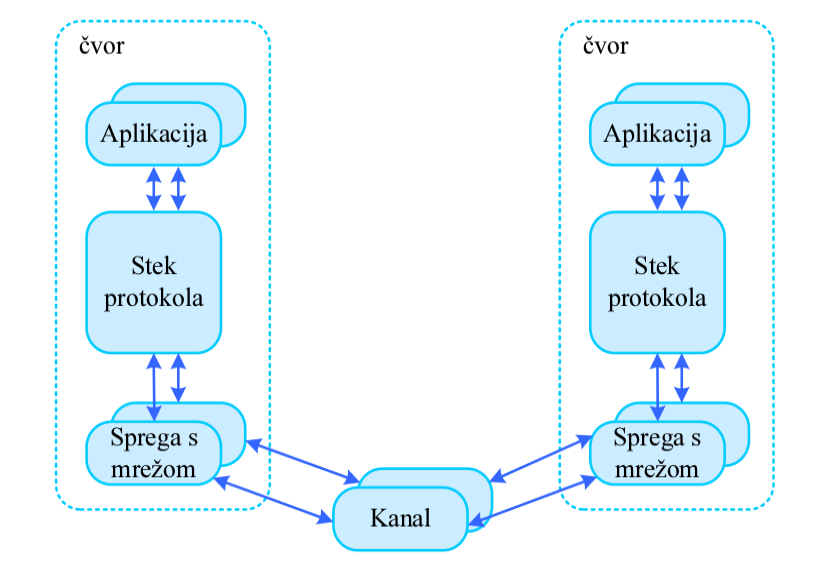
\includegraphics[width=.7\textwidth]{slike/nov.png}
\caption{\emp{Organizacija simulacionog modela u ns-3.}}
\label{fig:organizacija}
\end{figure}
\chapter{Dinami\v cko rutiranje}
\section{Zadatak}
U mre\v zi sa slike , izvor on-off TCP saobra\' caja je priklju\v cen na \v cvor n0, a primalac na \v cvor n4. Parametri linkova su dati u tabeli 2.1 \label(tab:par).
\begin{figure}[htb]
\centering
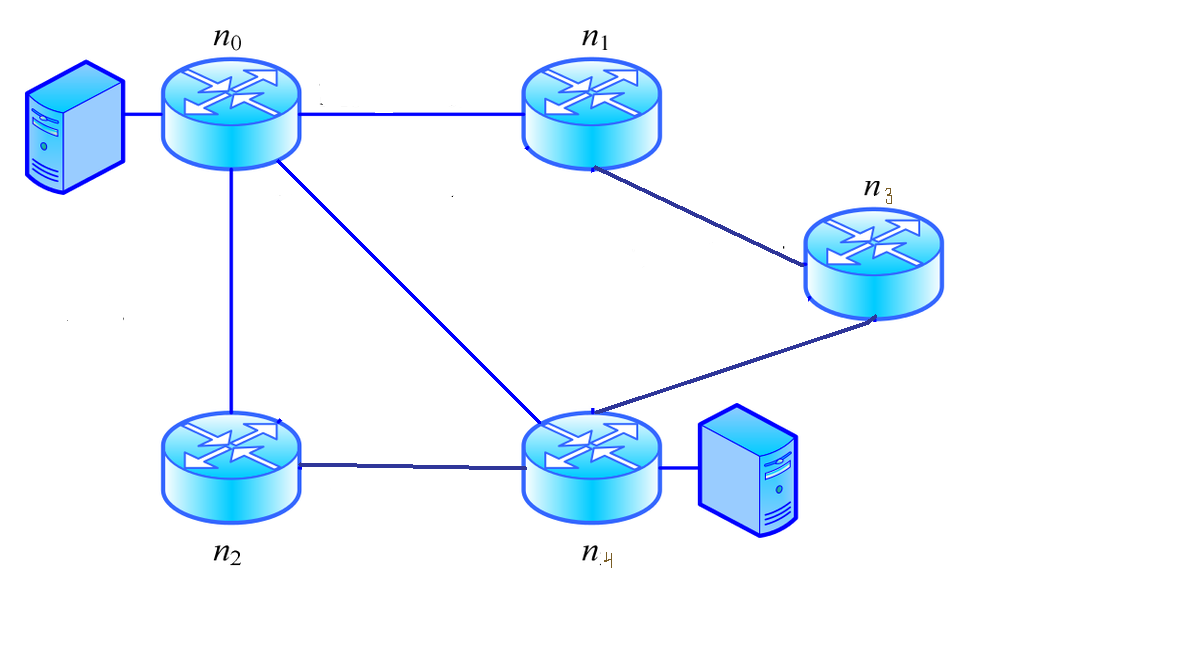
\includegraphics[width=.7\textwidth]{slike/nov1.png}
\caption{\emp{Izgled topologije mre\v ze.}}
\label{fig:organizacija}
\end{figure}

\begin{table}[htb]
\centering
\caption{Parametri linkova}
\medskip
\label{tab:par}
\begin{tabular}{c|c c c}
\hline
Link & Kapacitet & Propagaciono ka\v snjenje & Metrika\\
\hline
n0-n1 & 10 Mb/s & 4 ms & 4\\
\hline
n0-n2 & 10 Mb/s & 4 ms & 2\\
\hline
n0-n4 & 10 Mb/s & 3 ms & 6\\
\hline
n1-n3 & 10 Mb/s & 2 ms & 2\\
\hline
n2-n4 & 10 Mb/s & 2 ms & 1\\
\hline
n3-n4 & 10 Mb/s & 2 ms & 3\\
\end{tabular}
\end{table}


Posmatra se slede\' ci scenario de\v savanja:
\begin{itemize}
\item u trenutku t=1s,izvor po\v cinje emitovati saobra\v caj vr\v snim protokom 100 kb/s,
uz veli\v cinu TCP paketa 150 B,
\item u trenutku t =2 s, ukida se link izmedju \v cvorova n2 i n4 ,
\item u trenutku t =3 s, ukida se link izmedju \v cvorova n0 i n4 ,
\item u trenutku t =4 s, ponovo se uspostavlja link izmedju \v cvorova n2 i n4
\item u trenutku t =5 s, isklju\v cuje se izvor.\\
\end
Simullacijom je potrebno odrediti putanje saobra\' caja
\section{Opis simulacije}
Da bismo ilustrovali razli\ cite mogu\' cnosti konfigurisanja simulacionog modela u ns-3, izvor saobra\' caja smo pridru\v zili postoje\' cem \v cvoru mre\v ze  n 0 , u vidu OnOff aplikacije, dok smo prijemnik paketa (PacketSink) pridru\ zili novom \ cvoru n5. \v Cvorovi n4 i 5 povezani su linkom zanemarivog ka2njenja, kome dodeljujemo IP adrese iz opsega 164.70.7.0/24.\\
Metodom SetMetric zadajmo metriku linkova.Primetimo da se, iako su linkovi ,,ta\v cka-ta\v cka'' dvosmerni, mogu
zadati razli\v cite vrednosti metrike za dva smera prenosa.\\
Dogadjaji tokom izvr\v savanja simulacije se specifciraju metodom
Simulator::Schedule .
U na\v sem slu\v cju, njen poslednji argument se odnosi na indeks posmatranog mre\v znog
interfejsa, pri \v cemu 0 odgovara tzv.
loopback
interfejsu, dok su interfejsi ka fizi\v ckim
linkovima numerisani po redu kojim su pravljeni. Zanimljivo je da se linkovi ne isklju\v cuju direktno, ve\' c raskidanjem veze protokolskog steka
sa mre\v znim interfejsom.\\
Izve\v staje \' cemo snimiti kao
trace, pcap i xml
datoteke, a sa\v cuva\' cemo i tabele rutiranja posle
karakteristi£nih dogadjaja u mre\v zi. Na po\v cetku programa moramo eksplicitno tra\v ziti
da se tabele rutiranja a\v zuriraju posle svake promene stanja linkova, tako \v sto \' cemo
vrednost parametra ns3::Ipv4GlobalRouting::RespondToInterfaceEvents
postaviti na true .
\newpage
\section{Kod re\v senja}
\begin{verbatim}
#include <iostream>
#include <fstream>
#include <string>
#include <cassert>

#include "ns3/core-module.h"
#include "ns3/internet-module.h"
#include "ns3/point-to-point-module.h"
#include "ns3/network-module.h"
#include "ns3/applications-module.h"
#include "ns3/ipv4-global-routing-helper.h"
#include "ns3/netanim-module.h"
using namespace ns3;

int main (int argc, char *argv[])
{	

	// zadajemo azuriranje tabela rutiranja posle svake izmene stanja linka:
	Config::SetDefault ("ns3::Ipv4GlobalRouting::RespondToInterfaceEvents",
	BooleanValue (true));
	
	
	// pravimo cvorove:
	
	NodeContainer c;
	c.Create (6);
	
	// instaliramo stek protokola na cvorovima:	
	
	InternetStackHelper internet;
	internet.Install (c);
	
	NodeContainer n0n1 = NodeContainer (c.Get (0), c.Get (1));
	NodeContainer n0n2 = NodeContainer (c.Get (0), c.Get (2));
	NodeContainer n0n4 = NodeContainer (c.Get (0), c.Get (4));
	NodeContainer n1n3 = NodeContainer (c.Get (1), c.Get (3));
	NodeContainer n2n4 = NodeContainer (c.Get (2), c.Get (4));
	NodeContainer n3n4 = NodeContainer (c.Get (3), c.Get (4));
	NodeContainer n4n5 = NodeContainer (c.Get (4), c.Get (5));
	
	// pravimo linkove:
	PointToPointHelper p2p;

	p2p.SetDeviceAttribute ("DataRate", StringValue ("10Mbps"));
	p2p.SetChannelAttribute ("Delay", StringValue ("4ms"));
	
	//instaliranje linka izmedju cvorova
	NetDeviceContainer d0d1 = p2p.Install (n0n1);
	NetDeviceContainer d0d2 = p2p.Install (n0n2);
	p2p.SetChannelAttribute ("Delay", StringValue ("3ms"));

	NetDeviceContainer d0d4 = p2p.Install (n0n4);
	
	p2p.SetChannelAttribute ("Delay", StringValue ("2ms"));

	NetDeviceContainer d1d3 = p2p.Install (n1n3);
	NetDeviceContainer d2d4 = p2p.Install (n2n4);
	NetDeviceContainer d3d4 = p2p.Install (n3n4);

	p2p.SetChannelAttribute ("Delay", StringValue ("0ms"));
	NetDeviceContainer d4d5 = p2p.Install (n4n5);
	
	// dodeljujemo IP adrese:
	
	Ipv4AddressHelper ipv4;

	ipv4.SetBase ("164.70.1.0", "255.255.255.0");
	Ipv4InterfaceContainer i0i1 = ipv4.Assign (d0d1);
	ipv4.SetBase ("164.70.2.0", "255.255.255.0");
	Ipv4InterfaceContainer i0i2 =ipv4.Assign (d0d2);
	ipv4.SetBase ("164.70.3.0", "255.255.255.0");
	Ipv4InterfaceContainer i0i4 =ipv4.Assign (d0d4);
	ipv4.SetBase ("164.70.4.0", "255.255.255.0");
	Ipv4InterfaceContainer i1i3 =ipv4.Assign (d1d3);
	ipv4.SetBase ("164.70.5.0", "255.255.255.0");
	Ipv4InterfaceContainer i2i4 = ipv4.Assign (d2d4);
	ipv4.SetBase ("164.70.6.0", "255.255.255.0");
	Ipv4InterfaceContainer i3i4 = ipv4.Assign (d3d4);
	ipv4.SetBase ("164.70.7.0", "255.255.255.0");
	Ipv4InterfaceContainer i4i5 = ipv4.Assign (d4d5);


	// zadajemo metrike linkova
	// (pretpostavljena vrednost je 1):

	i0i1.SetMetric (0, 4);
	i0i1.SetMetric (1, 4);
	i0i2.SetMetric (0, 2);
	i0i2.SetMetric (1, 2);
	i0i4.SetMetric (0, 6);
	i0i4.SetMetric (1, 6);
	i1i3.SetMetric (0, 2);
	i1i3.SetMetric (1, 2);
	i3i4.SetMetric (0, 3);
	i3i4.SetMetric (1, 3);

	// pravimo tabele rutiranja:
	

	Ipv4GlobalRoutingHelper::PopulateRoutingTables ();
	

	// pravimo izvor saobracaja
	// i instaliramo ga na cvor 0:

	uint16_t port = 4001;
	OnOffHelper onoff ("ns3::TcpSocketFactory",InetSocketAddress (i4i5.GetAddress (1), port));
	onoff.SetAttribute ("OnTime",  StringValue("ns3::ConstantRandomVariable[Constant=100.0]"));
	onoff.SetAttribute ("OffTime",  StringValue("ns3::ConstantRandomVariable[Constant=0.0]"));
	onoff.SetAttribute ("DataRate", StringValue ("100kbps"));
	onoff.SetAttribute ("PacketSize", UintegerValue (150));

	ApplicationContainer apps = onoff.Install (c.Get (0));
	
	apps.Start (Seconds (1.0));
	apps.Stop (Seconds (5.0));

	// pravimo prijemnik saobracaja
	// i instaliramo ga na cvor 4:

	PacketSinkHelper sink ("ns3::TcpSocketFactory",Address (InetSocketAddress(Ipv4Address::GetAny (), port)));

	apps = sink.Install (c.Get (5));
	apps.Start (Seconds (1.0));
	apps.Stop (Seconds (5.0));

	// zadajemo snimanje izvestaja:
	
	AsciiTraceHelper ascii;
	Ptr<OutputStreamWrapper> stream = ascii.CreateFileStream ("dinamicko.tr");
	p2p.EnableAsciiAll (stream);
	internet.EnableAsciiIpv4All (stream);

	p2p.EnablePcapAll ("dinamicko");

	// postavljamo pointere:

	Ptr<Node> n0 = c.Get (0);
	Ptr<Ipv4> ipv4n0 = n0->GetObject<Ipv4> ();
	Ptr<Node> n2 = c.Get (2);
	Ptr<Ipv4> ipv4n2 = n2->GetObject<Ipv4> ();


	// u t = 2 s iskljucujemo link n2-n4:

	Simulator::Schedule (Seconds (2), &Ipv4::SetDown, ipv4n2, 2);

	// u t = 3 s iskljucujemo link n0-n4:

	Simulator::Schedule (Seconds (3), &Ipv4::SetDown, ipv4n0, 3);

 	// u t = 4 s ukljucujemo link n1-n2:
	
	Simulator::Schedule (Seconds (4), &Ipv4::SetUp, ipv4n2, 2);

	// snimamo tabele rutiranja:

	Ipv4GlobalRoutingHelper g;
	Ptr<OutputStreamWrapper> routingStream =Create<OutputStreamWrapper> ("dinamicko.routes", std::ios::out);

	g.PrintRoutingTableAllAt (Seconds (1), routingStream);
	g.PrintRoutingTableAllAt (Seconds (2), routingStream);
	g.PrintRoutingTableAllAt (Seconds (3), routingStream);
	g.PrintRoutingTableAllAt (Seconds (4), routingStream);
	g.PrintRoutingTableAllAt (Seconds (5), routingStream);

	//NetAnim
	std::string animFile = "dini.xml";
	AnimationInterface anim(animFile);
	// postavljamo potrebne pointere
	Ptr<Node> n1 = c.Get(1);
	Ptr<Node> n3 = c.Get(3);
	Ptr<Node> n4 = c.Get(4);
	Ptr<Node> n5 = c.Get(5);
	// zadajemo poziciju cvora n0 u NetAnim animaciji
	anim.SetConstantPosition( n0, 100, 100);
	anim.SetConstantPosition( n1, 200, 100);
	anim.SetConstantPosition( n2, 100, 200);
	anim.SetConstantPosition( n3, 200, 200);
	anim.SetConstantPosition( n4, 300, 150);
	anim.SetConstantPosition( n5, 300, 200);
	
	
	// pokre\' cemo simulaciju
	// i po njenom zavrsetku uni\v stavamo sve napravljene objekte:

	Simulator::Run ();
	Simulator::Destroy ();
}
\end{verbatim}
\section{Rezultati}
Razmotrimo sada analizu rezultata koje dobijamo po izvr\v savanju simulacije.
Primenjeni protokol rutiranja (OSPF) bira rutu ka odredi\v stu koja ima najmanju metriku; na po\v cetku je to n0 - n2 - n4 -n5.Kada u trenutku t = 2 s bude ispao link n2-n4, sabra\' caj \' ce se preusmeriti na rutu n0 - n4 - n5. U trenutku t = 3 s ispada i link izmedju \v cvorova n0-n4, nova putanja \' ce bii n0-n1-n3-n4-n5. Kada se u trenutu t = 4 s bude ponovo uspostavio link izmedju \v cvorova n 2 i n 2 , saobra\ caj \' ce se vratiti na prvobitnu putanju n 0 - n2 - n4 - n 5 .

Gornja zapa\v zanja potvrdjuju i tabele rutranja, koje zbog obimnosti navodimo samo za
\v cvor 0 u trenucima t =1s, t =2 s i t=3s.
\begin{verbatim}
Node: 0 Time: 1s Ipv4ListRouting table
  Priority: 0 Protocol: ns3::Ipv4StaticRouting
Destination     Gateway         Genmask         Flags Metric Ref    Use Iface
127.0.0.0       0.0.0.0         255.0.0.0       U     0      -      -   0
164.70.1.0      0.0.0.0         255.255.255.0   U     0      -      -   1
164.70.2.0      0.0.0.0         255.255.255.0   U     0      -      -   2
164.70.3.0      0.0.0.0         255.255.255.0   U     0      -      -   3
  Priority: -10 Protocol: ns3::Ipv4GlobalRouting
Destination     Gateway         Genmask         Flags Metric Ref    Use Iface
164.70.2.2      164.70.2.2      255.255.255.255 UH    -      -      -   2
164.70.5.1      164.70.2.2      255.255.255.255 UH    -      -      -   2
164.70.3.2      164.70.2.2      255.255.255.255 UH    -      -      -   2
164.70.5.2      164.70.2.2      255.255.255.255 UH    -      -      -   2
164.70.6.2      164.70.2.2      255.255.255.255 UH    -      -      -   2
164.70.7.1      164.70.2.2      255.255.255.255 UH    -      -      -   2
164.70.1.2      164.70.1.2      255.255.255.255 UH    -      -      -   1
164.70.4.1      164.70.1.2      255.255.255.255 UH    -      -      -   1
164.70.7.2      164.70.2.2      255.255.255.255 UH    -      -      -   2
164.70.4.2      164.70.1.2      255.255.255.255 UH    -      -      -   1
164.70.4.2      164.70.2.2      255.255.255.255 UH    -      -      -   2
164.70.6.1      164.70.1.2      255.255.255.255 UH    -      -      -   1
164.70.6.1      164.70.2.2      255.255.255.255 UH    -      -      -   2
127.0.0.0       164.70.2.2      255.0.0.0       UG    -      -      -   2
164.70.2.0      164.70.2.2      255.255.255.0   UG    -      -      -   2
164.70.5.0      164.70.2.2      255.255.255.0   UG    -      -      -   2
127.0.0.0       164.70.2.2      255.0.0.0       UG    -      -      -   2
164.70.3.0      164.70.2.2      255.255.255.0   UG    -      -      -   2
164.70.5.0      164.70.2.2      255.255.255.0   UG    -      -      -   2
164.70.6.0      164.70.2.2      255.255.255.0   UG    -      -      -   2
164.70.7.0      164.70.2.2      255.255.255.0   UG    -      -      -   2
127.0.0.0       164.70.2.2      255.0.0.0       UG    -      -      -   2
164.70.7.0      164.70.2.2      255.255.255.0   UG    -      -      -   2
127.0.0.0       164.70.1.2      255.0.0.0       UG    -      -      -   1
127.0.0.0       164.70.2.2      255.0.0.0       UG    -      -      -   2
164.70.4.0      164.70.1.2      255.255.255.0   UG    -      -      -   1
164.70.4.0      164.70.2.2      255.255.255.0   UG    -      -      -   2
164.70.6.0      164.70.1.2      255.255.255.0   UG    -      -      -   1
164.70.6.0      164.70.2.2      255.255.255.0   UG    -      -      -   2
127.0.0.0       164.70.1.2      255.0.0.0       UG    -      -      -   1
164.70.1.0      164.70.1.2      255.255.255.0   UG    -      -      -   1
164.70.4.0      164.70.1.2      255.255.255.0   UG    -      -      -   1

Node: 0 Time: 2s Ipv4ListRouting table
  Priority: 0 Protocol: ns3::Ipv4StaticRouting
Destination     Gateway         Genmask         Flags Metric Ref    Use Iface
127.0.0.0       0.0.0.0         255.0.0.0       U     0      -      -   0
164.70.1.0      0.0.0.0         255.255.255.0   U     0      -      -   1
164.70.2.0      0.0.0.0         255.255.255.0   U     0      -      -   2
164.70.3.0      0.0.0.0         255.255.255.0   U     0      -      -   3
  Priority: -10 Protocol: ns3::Ipv4GlobalRouting
Destination     Gateway         Genmask         Flags Metric Ref    Use Iface
164.70.2.2      164.70.2.2      255.255.255.255 UH    -      -      -   2
164.70.1.2      164.70.1.2      255.255.255.255 UH    -      -      -   1
164.70.4.1      164.70.1.2      255.255.255.255 UH    -      -      -   1
164.70.3.2      164.70.3.2      255.255.255.255 UH    -      -      -   3
164.70.6.2      164.70.3.2      255.255.255.255 UH    -      -      -   3
164.70.7.1      164.70.3.2      255.255.255.255 UH    -      -      -   3
164.70.4.2      164.70.1.2      255.255.255.255 UH    -      -      -   1
164.70.6.1      164.70.1.2      255.255.255.255 UH    -      -      -   1
164.70.7.2      164.70.3.2      255.255.255.255 UH    -      -      -   3
127.0.0.0       164.70.2.2      255.0.0.0       UG    -      -      -   2
164.70.2.0      164.70.2.2      255.255.255.0   UG    -      -      -   2
127.0.0.0       164.70.1.2      255.0.0.0       UG    -      -      -   1
164.70.1.0      164.70.1.2      255.255.255.0   UG    -      -      -   1
164.70.4.0      164.70.1.2      255.255.255.0   UG    -      -      -   1
127.0.0.0       164.70.1.2      255.0.0.0       UG    -      -      -   1
164.70.4.0      164.70.1.2      255.255.255.0   UG    -      -      -   1
164.70.6.0      164.70.1.2      255.255.255.0   UG    -      -      -   1
127.0.0.0       164.70.3.2      255.0.0.0       UG    -      -      -   3
164.70.3.0      164.70.3.2      255.255.255.0   UG    -      -      -   3
164.70.5.0      164.70.3.2      255.255.255.0   UG    -      -      -   3
164.70.6.0      164.70.3.2      255.255.255.0   UG    -      -      -   3
164.70.7.0      164.70.3.2      255.255.255.0   UG    -      -      -   3
127.0.0.0       164.70.3.2      255.0.0.0       UG    -      -      -   3
164.70.7.0      164.70.3.2      255.255.255.0   UG    -      -      -   3

Node: 0 Time: 3s Ipv4ListRouting table
  Priority: 0 Protocol: ns3::Ipv4StaticRouting
Destination     Gateway         Genmask         Flags Metric Ref    Use Iface
127.0.0.0       0.0.0.0         255.0.0.0       U     0      -      -   0
164.70.1.0      0.0.0.0         255.255.255.0   U     0      -      -   1
164.70.2.0      0.0.0.0         255.255.255.0   U     0      -      -   2
  Priority: -10 Protocol: ns3::Ipv4GlobalRouting
Destination     Gateway         Genmask         Flags Metric Ref    Use Iface
164.70.2.2      164.70.2.2      255.255.255.255 UH    -      -      -   2
164.70.1.2      164.70.1.2      255.255.255.255 UH    -      -      -   1
164.70.4.1      164.70.1.2      255.255.255.255 UH    -      -      -   1
164.70.4.2      164.70.1.2      255.255.255.255 UH    -      -      -   1
164.70.6.1      164.70.1.2      255.255.255.255 UH    -      -      -   1
164.70.6.2      164.70.1.2      255.255.255.255 UH    -      -      -   1
164.70.7.1      164.70.1.2      255.255.255.255 UH    -      -      -   1
164.70.7.2      164.70.1.2      255.255.255.255 UH    -      -      -   1
127.0.0.0       164.70.2.2      255.0.0.0       UG    -      -      -   2
164.70.2.0      164.70.2.2      255.255.255.0   UG    -      -      -   2
127.0.0.0       164.70.1.2      255.0.0.0       UG    -      -      -   1
164.70.1.0      164.70.1.2      255.255.255.0   UG    -      -      -   1
164.70.4.0      164.70.1.2      255.255.255.0   UG    -      -      -   1
127.0.0.0       164.70.1.2      255.0.0.0       UG    -      -      -   1
164.70.4.0      164.70.1.2      255.255.255.0   UG    -      -      -   1
164.70.6.0      164.70.1.2      255.255.255.0   UG    -      -      -   1
127.0.0.0       164.70.1.2      255.0.0.0       UG    -      -      -   1
164.70.3.0      164.70.1.2      255.255.255.0   UG    -      -      -   1
164.70.5.0      164.70.1.2      255.255.255.0   UG    -      -      -   1
164.70.6.0      164.70.1.2      255.255.255.0   UG    -      -      -   1
164.70.7.0      164.70.1.2      255.255.255.0   UG    -      -      -   1
127.0.0.0       164.70.1.2      255.0.0.0       UG    -      -      -   1
164.70.7.0      164.70.1.2      255.255.255.0   UG    -      -      -   1

\end{verbatim}
U trenutku
t =1 s, najbolje  rute iz \v cvora n0 ka svim ostaim \v clanovima idu preko intrfejsa 
interfejsa 2, koji vodi ka \v cvoru n2. U trenutku t= 2 , ispada lik izmedju \v cvorova n2 i n4. U tabeli rutiranja \v cvora n0 stoga \' ce rute ka \v cvoru 4 i\' ci preko interfejsa 3.

\chapter{Animacija rezultata simulacije}
\section{NetAnim}
Animator NetAnim je namenje radu s C++ programskim skriptama. Da bismo mogu\v cili animaciju rezultata na\v seg programa, pozivmo na\v etku modul netanim
\begin{verbatim}
#include "ns3/netanim-module.h"
\end{verbatim}
Potom defini\v semo izlaznu xml datoteku i polo\v zaje \v cvorova, kao \v sto je prikazano u kodu u poglavlju 2.3.\\
Nakon izv\v savanja simulacije, u osnonom direktorijumu se pravi datoteka dini.xml .
Kada je budemo otvorili u programu NetAnim, vide¢emo slede¢u sliku:\label{fig:stanje0}
\begin{figure}[htb]
\centering
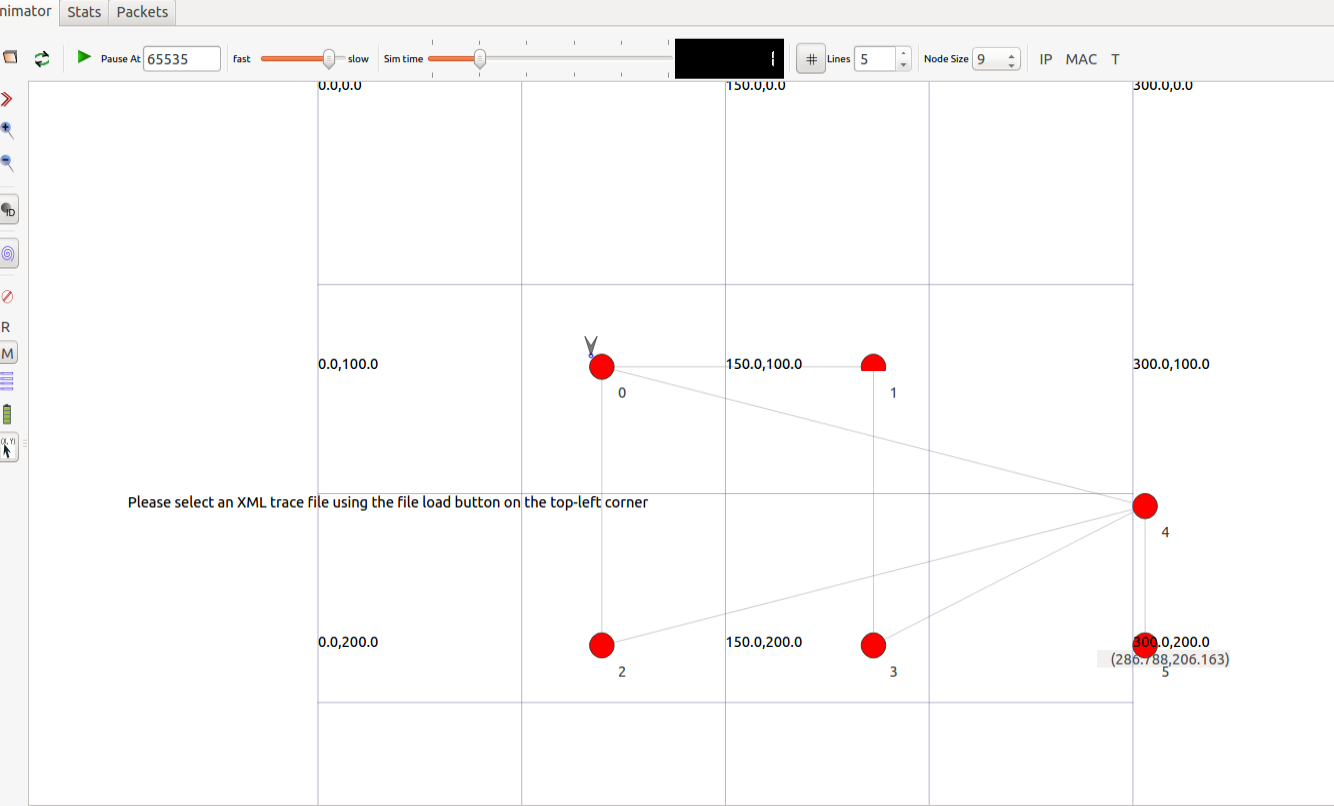
\includegraphics[width=.7\textwidth]{slike/0.png}
\caption{\emp{Po\v cetno stanje mre\v ze.}}
\label{fig:stanje0}
\end{figure}

Pokretanjem animacije, vide\' cemo tokove paketa po linkovima. Prikazi u karakteristi\ cnim trenucima dati su na slici \label{fig:stanje1}
\begin{figure}[htb]
\centering
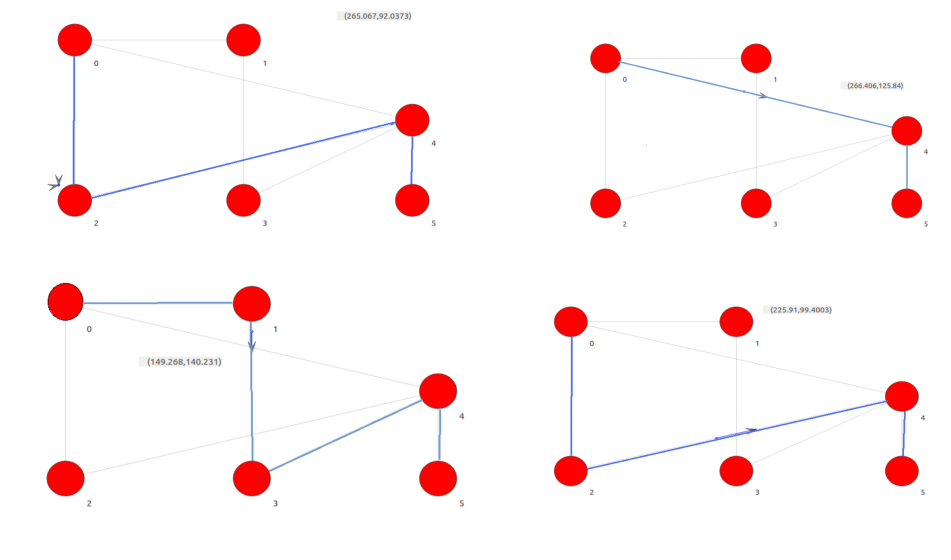
\includegraphics[width=.7\textwidth]{slike/1.png}
\caption{\emp{Stanje mre\v ze u trenucima 1s, 2s, 3s i 4s respektivno.}}
\label{fig:stanje1}
\end{figure}
\chapter{Zaklju\v cak}

U radu je prkazan prenos TCP paketa kroz mre\v zu odredjene topologije uz izmenu stanja u mre\v zi  u odredjenim trenucima. Cilj je bio da koriste\v ci vec implementirane klase i metode, koje nam pru\v za ns-3, prika\v zemo pona\v sanje mre\v ze tokom prenosa paketa kroz nju. Dato re\v senje e mo\v ze e nadogradjiti u smislu pove\v canja broja \v cvorova, promeni topologije ili pak promeni tipa paketa koji se prenosi.


\renewcommand{\bibname}{Literatura}
\begin{thebibliography}{100}


\bibitem{1} Dr Milan Bjelica \textbf{MODELIRANJE I SIMULACIJA U TELEKOMUNIKACIJAMA}, Beograd 2013., Elektrotehni\v cki fakultet

\bibitem{2} Asistent dr Nata\v sa Maksi\' c, \textbf{Mre\v zni simulator ns-3}, Elektrotehni\v cki fakultet.\\

\end{thebibliography}

\end{document}
